%%%%%%%%%%%%%%%%%%%%%%%%%%%%%%%%%%%%%%%%%
% Daily Laboratory Book
% LaTeX Template
%
% This template has been downloaded from:
% http://www.latextemplates.com
%
% Original author:
% Frank Kuster (http://www.ctan.org/tex-archive/macros/latex/contrib/labbook/)
%
% Important note:
% This template requires the labbook.cls file to be in the same directory as the
% .tex file. The labbook.cls file provides the necessary structure to create the
% lab book.
%
% The \lipsum[#] commands throughout this template generate dummy text
% to fill the template out. These commands should all be removed when 
% writing lab book content.
%
% HOW TO USE THIS TEMPLATE 
% Each day in the lab consists of three main things:
%
% 1. LABDAY: The first thing to put is the \labday{} command with a date in 
% curly brackets, this will make a new page and put the date in big letters 
% at the top.
%
% 2. EXPERIMENT: Next you need to specify what experiment(s) you are 
% working on with an \experiment{} command with the experiment shorthand 
% in the curly brackets. The experiment shorthand is defined in the 
% 'DEFINITION OF EXPERIMENTS' section below, this means you can 
% say \experiment{pcr} and the actual text written to the PDF will be what 
% you set the 'pcr' experiment to be. If the experiment is a one off, you can 
% just write it in the bracket without creating a shorthand. Note: if you don't 
% want to have an experiment, just leave this out and it won't be printed.
%
% 3. CONTENT: Following the experiment is the content, i.e. what progress 
% you made on the experiment that day.
%
%%%%%%%%%%%%%%%%%%%%%%%%%%%%%%%%%%%%%%%%%

%----------------------------------------------------------------------------------------
%	PACKAGES AND OTHER DOCUMENT CONFIGURATIONS
%----------------------------------------------------------------------------------------

\documentclass[idxtotoc,hyperref,openany]{labbook} % 'openany' here removes the gap page between days, erase it to restore this gap; 'oneside' can also be added to remove the shift that odd pages have to the right for easier reading

\usepackage[ 
  backref=page,
  pdfpagelabels=true,
  plainpages=false,
  colorlinks=true,
  bookmarks=true,
  pdfview=FitB]{hyperref} % Required for the hyperlinks within the PDF

\usepackage[brazilian]{babel}  
\usepackage{booktabs} % Required for the top and bottom rules in the table
\usepackage{float} % Required for specifying the exact location of a figure or table
\usepackage{graphicx} % Required for including images
\usepackage{lipsum} % Used for inserting dummy 'Lorem ipsum' text into the template
\usepackage[utf8]{inputenc}

\usepackage[T1]{fontenc} % Permite copiar e colar textos do PDF para outros locais, sem desformatar os caracteres acentuados
\usepackage[separate-uncertainty=true,multi-part-units=single]{siunitx} %Inserir unidades no SI de maneira formatada
\usepackage[parfill]{parskip} %Include empty line between paragraphs


\newcommand{\HRule}{\rule{\linewidth}{0.5mm}} % Command to make the lines in the title page
\setlength\parindent{0pt} % Removes all indentation from paragraphs

%----------------------------------------------------------------------------------------
%	DEFINITION OF EXPERIMENTS
%----------------------------------------------------------------------------------------

\newexperiment{simulation}{Simulação}
\newexperiment{data}{Análise de Dados}
\newexperiment{gui}{Programação da GUI}
\newexperiment{writing}{Escrita do TCC}
\newexperiment{table}{This shows a sample table}
%\newexperiment{shorthand}{Description of the experiment}

%---------------------------------------------------------------------------------------

\begin{document}

%----------------------------------------------------------------------------------------
%	TITLE PAGE
%----------------------------------------------------------------------------------------

\frontmatter % Use Roman numerals for page numbers
\title{
\begin{center}
\HRule \\[0.4cm]
{\Huge \bfseries Laboratory Journal \\[0.5cm] \Large Trabalho de Conclusão de Curso}\\[0.4cm] % Degree
\HRule \\[1.5cm]
\end{center}
}
\author{\Huge Yuri R. Tonin \\ \\ \LARGE yuri@df.ufscar.br \\[2cm]} % Your name and email address
\date{Início do Journal: 31 de Outubro de 2017} % Beginning date
\maketitle

\tableofcontents

\mainmatter % Use Arabic numerals for page numbers

%----------------------------------------------------------------------------------------
%	LAB BOOK CONTENTS
%----------------------------------------------------------------------------------------

% Blank template to use for new days:

%\labday{Day, Date Month Year}

%\experiment{}

%Text

%-----------------------------------------

%\experiment{}

%Text

%----------------------------------------------------------------------------------------

\labday{Terça, 31 de Outubro de 2017}

\experiment{data}


Ao realizar simulações, observamos que um sinal com um ruído aleatório (de distribuição gaussiana e largura 1 desvio padrão) causava uma grande incerteza na posição dos pontos da curva linear (figura \ref{fig:linearcurve}). O comportamento esperado é que o ponto a esquerda representa o ângulo maior (no caso, $\SI{10}{\degree})$, enquanto que o outro represente o ângulo menor ($\SI{2}{\degree}$). As simulações mostravam caso em que as posições se invertiam, devido ao grande ruído. 

Seja $S$ o sinal. No eixo Y, plota-se $S/\sin$. No eixo X, $S/\tan$. Espera-se que $S / \sin(\SI{2}{\degree}) > S_{10} / \sin(\SI{10}{\degree})$ pois o numerador cresce menos que o denominador quando se muda o ângulo de $\SI{2}{\degree}$ para $\SI{2}{\degree}$. Para ver isso basta plotar uma curva do sinal ideal e ver a variação em cada valor dos ângulos.


\begin{figure}[H]
	\begin{center}
		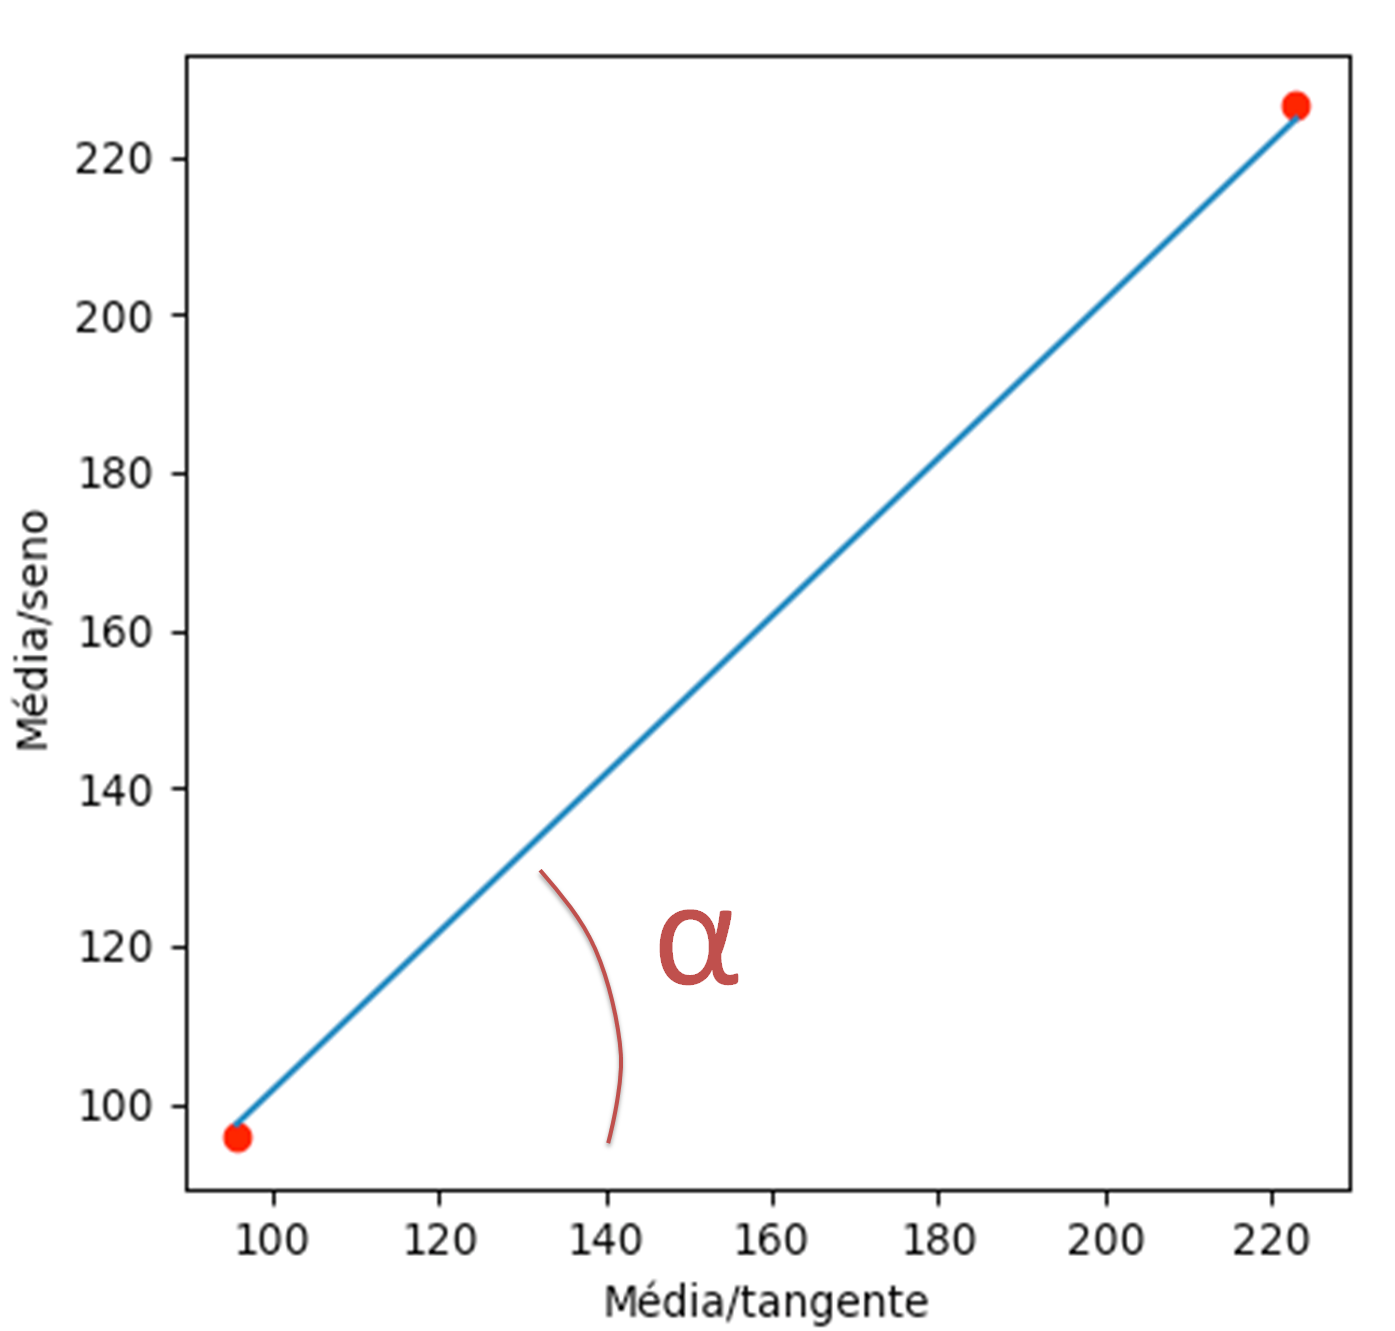
\includegraphics[width=0.5\linewidth]{linearcurve}
	\end{center}
	\caption{}
	\label{fig:linearcurve}
\end{figure}


Voltamos então a GUI para avaliar se os fittings também apresentavam o mesmo comportamento. Descobrimos que os valores estavam sempre invertidos, isto é, o ponto da esquerda era o de $\SI{2}{\degree}$ e o da direita de $\SI{10}{\degree}$. O motivo é que o valor de $S_{10} >> S_2$. Isso não pode estar correto. Portanto, tudo indica que há uma diferença de ganho no sinal em diferentes aquisições, já que um conjunto de dados com determinado ângulo diz respeito UMA aquisição.

Iremos então realizar uma análise dessa diferença no sinal para cada um dos ângulo. Usaremos a GUI para dados de diversos pacientes e analisaremos a inclinação da reta é aproximadamente a mesma para todos os pacientes. se houver uma consistência, poderemos fazer o mesmo para uma região de gorda (onde o contraste não atinge) e outra de rim (por onde o contraste passa). Essas regiões poderão ser utilizadas como referência para criarmos um ``segundo rescaling'' e obter os valores corretos (ou mais próximos dos corretos) para a média de uma ROI (sinal).

\experiment{data}

O Fernando me passou os dados de diversos pacientes. Por agilidade, optamos por calcular as médias das ROIs pelo MIPAV. Fiz a análise de apenas 1 paciente para as imagens pré-contraste. Algo estranho aconteceu: as médias da ROI estão dando valores (muito!) diferentes do que quando calculo pela minha GUI do Python. E o pior: pelo MIPAV, a diferença de intensidade da imagem de 2 para a de 10 graus parece ser de 4 vezes, como deve ser! \textbf{Checar documentação do MIPAV} para ver se calculei corretamente as médias pelo software. Caso isso se confirme, terei que ver na GUI se fiz algum cálculo com a imagem que possa estar alterando os valores do pixels e mudando tanto assim a média do sinal na ROI. Também posso tentar entender como o Python importa as imagens; quem sabe na importação algo está alterando os valores...

ERRATA: O motivo para a diferença acima foi encontrado no dia seguinte.

\labday{Quarta, 1 de novembro de 2017}

\experiment{data}

A diferença nos valores do MIPAV e da GUI citadas ontem ocorrem por causa do rescaling que fiz na GUI. O MIPAV não faz o rescaling. Assim, extrai o valor dos coeficientes de rescaling pela GUI e vou implementar o rescaling pelo excel posteriormente após extrair todos os valores de intensidade pelo MIPAV.

\labday{Terça, 7 de novembro de 2017}

\experiment{data}

Terminei de analisar as médias do sinais provenientes de diferentes regiões: 3 do fígado, 1 do rim e 2 de gordura. 

Ignorei o SUBJ021 porque seu arquivo DICOM era único para todos os slices e assim não consegui extrair os Rescaling factors a partir da minha GUI, a qual precisa de 1 arquivo por slice.

A tabela \ref{tabelaMedias} mostra os valores do coeficiente angular da reta gerada pelos dois pontos de cada região (2 e 10 graus), para cada sujeito. 

Vemos que os SUBJ011 e SUBJ018 possuem valores bem altos para o coeficiente. Vemos que que as regiões de gordura possuem o menor desvio padrão. Todos os demais possuem desvio padrão da de 100\% da média.

A variação é considerável. Preciso falar com o Fernando e ver se poderemos fazer a análise que tinhamos em mente ou não.

EDIT: Dois pacientes (SUBJ011 e SUBJ018) apresentavam valores bem discrepantes do restante. Optamos por ignorar esses pontos. Ao ignorar esses pontos, a média e o desvio padrão melhoram consideravelmente (tabela 2). Vamos utilizar essa tabela sem esses 2 pacientes.

\begin{table}[]
	\centering
	\caption{Coeficiente angular entre os dois pontos de intensidade para diferente pacientes e regiões}
	\label{tabelaMedias}
	\begin{tabular}{ccccccc}
		\hline
		\multicolumn{1}{|c|}{\textbf{Paciente}} & \multicolumn{1}{c|}{\textbf{Fígado A}} & \multicolumn{1}{c|}{\textbf{Fígado B}} & \multicolumn{1}{c|}{\textbf{Fígado C}} & \multicolumn{1}{c|}{\textbf{Rim}} & \multicolumn{1}{c|}{\textbf{Gordura A}} & \multicolumn{1}{c|}{\textbf{Gordura B}} \\ \hline
		\multicolumn{1}{|c|}{\textbf{SUBJ001}}  & \multicolumn{1}{c|}{4.31}              & \multicolumn{1}{c|}{4.27}              & \multicolumn{1}{c|}{5.42}              & \multicolumn{1}{c|}{4.14}         & \multicolumn{1}{c|}{1.25}               & \multicolumn{1}{c|}{1.34}               \\ \hline
		\multicolumn{1}{|c|}{\textbf{SUBJ002}}  & \multicolumn{1}{c|}{4.78}              & \multicolumn{1}{c|}{4.00}              & \multicolumn{1}{c|}{4.08}              & \multicolumn{1}{c|}{2.55}         & \multicolumn{1}{c|}{1.41}               & \multicolumn{1}{c|}{1.41}               \\ \hline
		\multicolumn{1}{|c|}{\textbf{SUBJ003}}  & \multicolumn{1}{c|}{4.12}              & \multicolumn{1}{c|}{4.86}              & \multicolumn{1}{c|}{5.05}              & \multicolumn{1}{c|}{4.02}         & \multicolumn{1}{c|}{0.95}               & \multicolumn{1}{c|}{0.95}               \\ \hline
		\multicolumn{1}{|c|}{\textbf{SUBJ004}}  & \multicolumn{1}{c|}{4.11}              & \multicolumn{1}{c|}{3.73}              & \multicolumn{1}{c|}{4.33}              & \multicolumn{1}{c|}{2.20}         & \multicolumn{1}{c|}{0.87}               & \multicolumn{1}{c|}{0.87}               \\ \hline
		\multicolumn{1}{|c|}{\textbf{SUBJ005}}  & \multicolumn{1}{c|}{3.50}              & \multicolumn{1}{c|}{3.64}              & \multicolumn{1}{c|}{4.69}              & \multicolumn{1}{c|}{3.42}         & \multicolumn{1}{c|}{1.16}               & \multicolumn{1}{c|}{1.16}               \\ \hline
		\multicolumn{1}{|c|}{\textbf{SUBJ006}}  & \multicolumn{1}{c|}{5.89}              & \multicolumn{1}{c|}{6.97}              & \multicolumn{1}{c|}{7.05}              & \multicolumn{1}{c|}{3.51}         & \multicolumn{1}{c|}{1.52}               & \multicolumn{1}{c|}{1.52}               \\ \hline
		\multicolumn{1}{|c|}{\textbf{SUBJ007}}  & \multicolumn{1}{c|}{2.77}              & \multicolumn{1}{c|}{2.41}              & \multicolumn{1}{c|}{2.20}              & \multicolumn{1}{c|}{1.86}         & \multicolumn{1}{c|}{0.83}               & \multicolumn{1}{c|}{0.83}               \\ \hline
		\multicolumn{1}{|c|}{\textbf{SUBJ008}}  & \multicolumn{1}{c|}{4.51}              & \multicolumn{1}{c|}{4.73}              & \multicolumn{1}{c|}{5.42}              & \multicolumn{1}{c|}{3.07}         & \multicolumn{1}{c|}{1.02}               & \multicolumn{1}{c|}{1.02}               \\ \hline
		\multicolumn{1}{|c|}{\textbf{SUBJ009}}  & \multicolumn{1}{c|}{7.76}              & \multicolumn{1}{c|}{8.20}              & \multicolumn{1}{c|}{8.37}              & \multicolumn{1}{c|}{4.51}         & \multicolumn{1}{c|}{2.10}               & \multicolumn{1}{c|}{2.10}               \\ \hline
		\multicolumn{1}{|c|}{\textbf{SUBJ010}}  & \multicolumn{1}{c|}{4.14}              & \multicolumn{1}{c|}{4.56}              & \multicolumn{1}{c|}{4.82}              & \multicolumn{1}{c|}{2.77}         & \multicolumn{1}{c|}{0.96}               & \multicolumn{1}{c|}{0.96}               \\ \hline
		\multicolumn{1}{|c|}{\textbf{SUBJ011}}  & \multicolumn{1}{c|}{11.28}             & \multicolumn{1}{c|}{11.14}             & \multicolumn{1}{c|}{10.88}             & \multicolumn{1}{c|}{9.89}         & \multicolumn{1}{c|}{3.65}               & \multicolumn{1}{c|}{3.65}               \\ \hline
		\multicolumn{1}{|c|}{\textbf{SUBJ012}}  & \multicolumn{1}{c|}{4.13}              & \multicolumn{1}{c|}{3.58}              & \multicolumn{1}{c|}{4.12}              & \multicolumn{1}{c|}{2.18}         & \multicolumn{1}{c|}{1.46}               & \multicolumn{1}{c|}{1.46}               \\ \hline
		\multicolumn{1}{|c|}{\textbf{SUBJ013}}  & \multicolumn{1}{c|}{5.88}              & \multicolumn{1}{c|}{5.76}              & \multicolumn{1}{c|}{6.52}              & \multicolumn{1}{c|}{4.05}         & \multicolumn{1}{c|}{1.20}               & \multicolumn{1}{c|}{1.20}               \\ \hline
		\multicolumn{1}{|c|}{\textbf{SUBJ014}}  & \multicolumn{1}{c|}{5.36}              & \multicolumn{1}{c|}{5.31}              & \multicolumn{1}{c|}{5.09}              & \multicolumn{1}{c|}{3.01}         & \multicolumn{1}{c|}{1.12}               & \multicolumn{1}{c|}{1.12}               \\ \hline
		\multicolumn{1}{|c|}{\textbf{SUBJ015}}  & \multicolumn{1}{c|}{2.93}              & \multicolumn{1}{c|}{2.48}              & \multicolumn{1}{c|}{2.43}              & \multicolumn{1}{c|}{3.43}         & \multicolumn{1}{c|}{0.95}               & \multicolumn{1}{c|}{0.95}               \\ \hline
		\multicolumn{1}{|c|}{\textbf{SUBJ016}}  & \multicolumn{1}{c|}{2.95}              & \multicolumn{1}{c|}{2.74}              & \multicolumn{1}{c|}{2.49}              & \multicolumn{1}{c|}{2.33}         & \multicolumn{1}{c|}{0.95}               & \multicolumn{1}{c|}{0.95}               \\ \hline
		\multicolumn{1}{|c|}{\textbf{SUBJ017}}  & \multicolumn{1}{c|}{1.90}              & \multicolumn{1}{c|}{1.77}              & \multicolumn{1}{c|}{1.54}              & \multicolumn{1}{c|}{1.43}         & \multicolumn{1}{c|}{0.69}               & \multicolumn{1}{c|}{0.69}               \\ \hline
		\multicolumn{1}{|c|}{\textbf{SUBJ018}}  & \multicolumn{1}{c|}{29.18}             & \multicolumn{1}{c|}{30.10}             & \multicolumn{1}{c|}{31.92}             & \multicolumn{1}{c|}{36.99}        & \multicolumn{1}{c|}{3.87}               & \multicolumn{1}{c|}{3.87}               \\ \hline
		\multicolumn{1}{|c|}{\textbf{SUBJ019}}  & \multicolumn{1}{c|}{4.38}              & \multicolumn{1}{c|}{4.97}              & \multicolumn{1}{c|}{6.01}              & \multicolumn{1}{c|}{3.73}         & \multicolumn{1}{c|}{1.55}               & \multicolumn{1}{c|}{1.55}               \\ \hline
		\multicolumn{1}{|c|}{\textbf{SUBJ020}}  & \multicolumn{1}{c|}{2.61}              & \multicolumn{1}{c|}{3.07}              & \multicolumn{1}{c|}{2.84}              & \multicolumn{1}{c|}{1.89}         & \multicolumn{1}{c|}{0.84}               & \multicolumn{1}{c|}{0.84}               \\ \hline
		\multicolumn{1}{|c|}{\textbf{SUBJ022}}  & \multicolumn{1}{c|}{7.36}              & \multicolumn{1}{c|}{8.63}              & \multicolumn{1}{c|}{9.52}              & \multicolumn{1}{c|}{5.11}         & \multicolumn{1}{c|}{3.82}               & \multicolumn{1}{c|}{3.82}               \\ \hline
		\multicolumn{1}{|c|}{\textbf{SUBJ023}}  & \multicolumn{1}{c|}{2.75}              & \multicolumn{1}{c|}{2.63}              & \multicolumn{1}{c|}{2.97}              & \multicolumn{1}{c|}{2.37}         & \multicolumn{1}{c|}{1.18}               & \multicolumn{1}{c|}{1.18}               \\ \hline
		\textbf{}                               &                                        &                                        &                                        &                                   &                                         &                                         \\ \hline
		\multicolumn{1}{|c|}{\textbf{Average}}  & \multicolumn{1}{c|}{5.7539524}         & \multicolumn{1}{c|}{5.8894279}         & \multicolumn{1}{c|}{6.2617352}         & \multicolumn{1}{c|}{4.9292917}    & \multicolumn{1}{c|}{1.515662925}        & \multicolumn{1}{c|}{1.520010985}        \\ \hline
		\multicolumn{1}{|c|}{\textbf{StDev}}    & \multicolumn{1}{c|}{5.6343634}         & \multicolumn{1}{c|}{5.8704812}         & \multicolumn{1}{c|}{6.2014859}         & \multicolumn{1}{c|}{7.3660122}    & \multicolumn{1}{c|}{0.972241553}        & \multicolumn{1}{c|}{0.971191236}        \\ \hline
	\end{tabular}
\end{table}

\begin{table}[]
	\centering
	\caption{Valores da média e desvio padrão após retirada dos pacientes 11 e 18}
	\label{tabelaMedias2}
	\begin{tabular}{|c|c|c|c|c|c|c|}
		\hline
		\textbf{Average} & 4.31 & 4.42 & 4.75 & 3.08 & 1.29 & 1.30 \\ \hline
		\textbf{StDev}   & 1.55 & 1.87 & 2.08 & 0.99 & 0.68 & 0.58 \\ \hline
	\end{tabular}
\end{table}


\labday{Quarta, 8 de novembro de 2017}

\experiment{writing}

Terminei uma primeira parte da introdução teórica sobre os fundamentos físicos da RM. Preciso agora falar do sinal (SIL, Transformada de Fourier, etc). Como devo estruturar essa segunda parte?

\experiment{data}

Ao analisar os valores da tablea \ref{tabelaMedias2}, vemos que a variação do coeficiente angular existe mas não é tão grande. Ou seja, apesar do rescaling de cada aquisição (2 e 10) serem muito diferentes e causarem um valor ilógico na diferença de intensidade dos pontos, essa ``ilogicidade'' mantém-se aproximadamente a mesma para os diversos pacientes. Portanto, podemos tentar realizar um segundo rescaling que irá corrigir esse ``erro'' do rescaling introduzido pelo uso dos dados provenientes de aquisições distintas.

EDIT: Pelo paper de Garnov (2013), creio que podemos utilizar $T1_{gordura}=\SI{300}{\milli \second}$.

 \section*{Como realizaremos a correção:}
 
  Primeiramente, devemos o valor de $T_1$ para a gordura abdominal na literatura e assumir esse como o valor verdadeiro. Com esse valor, simularemos quantas vezes deve aumentar o sinal (fator $\alpha$) do ponto de $2^o$ para o ponto de $10^o$. Então, ajustaremos o dado da média de intensidade em $10^o$ para que este seja $\alpha$ vezes maior que o dado em $2^o$, isto é, multiplicaremos os dos dados por um fator $\beta$. Este novo fator será utilizado para ajustar os dados dos demais órgãos.
  
  Com os dados ajustados, iremos avaliar se as intensidades do fígado fornecem a posição correta dos pontos, como discutido no dia 31 de outubro de 2017. 


\labday{Quinta, 9 de novembro de 2017}

\experiment{data}

Simulei o sinal $\rho$ utilizando o tempo de relaxação da gordura $T1_{gordura} = 300 ms$. Os demais parâmetros foram os mesmos da imagem que tomamos como referência até o momento:

\begin{itemize}
	\item $T2 = 72 ms$
	\item $TE = 1.813 ms$
	\item $TR = 162.54 ms$
\end{itemize}

Após realizar a análise, observei que o fator era maior que 1 para alguns pacientes e menor para outros. Decidimos investigar mais a fundo. Fato é que, ao cancular S/sin e S/tan para todos os pacientes e obter o coeficiente angular após a linearização, temos que ALGUNS pacientes apresentam valores bons (S2 > S10). Em outros, o comportamento bom aparece apenas em uma região ou outra, enquanto é problemático nas demais.

\label{Sexta, 10 de novembro de 2017}

\experiment{data}

Mostrei os valores de T1 obtidos pelo Excel para o Fernando. Ele entendeu que o problema está nos valores dos ângulos utilizados e disse que irá pensar no que poderemos fazer. Enquanto isso, continuei a escrever o TCC.

%----------------------------------------------------------------------------------------
%	FORMULAE
%----------------------------------------------------------------------------------------

\newpage

\huge \textbf{Fórmulas} \\ \\

\normalsize \textbf{Formula 1 - Pythagorean theorem}\\ \\
$a^2 + b^2 = c^2$\\ \\

%-----------------------------------------

%\textbf{Formula X - Description}\\ \\

%Formula

%----------------------------------------------------------------------------------------

\end{document}